\documentclass[
11pt, % The default document font size, options: 10pt, 11pt, 12pt
%codirector, % Uncomment to add a codirector to the title page
]{charter} 


% El títulos de la memoria, se usa en la carátula y se puede usar el cualquier lugar del documento con el comando \ttitle
\titulo{Sistema de recomendación para retail aumentado por transfer learning} 

% Nombre del posgrado, se usa en la carátula y se puede usar el cualquier lugar del documento con el comando \degreename
%\posgrado{Carrera de Especialización en Sistemas Embebidos} 
%\posgrado{Carrera de Especialización en Internet de las Cosas} 
\posgrado{Carrera de Especialización en Inteligencia Artificial}
%\posgrado{Maestría en Sistemas Embebidos} 
%\posgrado{Maestría en Internet de las cosas}

% Tu nombre, se puede usar el cualquier lugar del documento con el comando \authorname
% IMPORTANTE: no omitir titulaciones ni tildación en los nombres, también se recomienda escribir los nombres completos (tal cual los tienen en su documento)
\autor{Lic. Matías Agustín Souto}

% El nombre del director y co-director, se puede usar el cualquier lugar del documento con el comando \supname y \cosupname y \pertesupname y \pertecosupname
\director{\textit{A definir}}
\pertenenciaDirector{\textit{A definir}} 
\codirector{} % para que aparezca en la portada se debe descomentar la opción codirector en los parámetros de documentclass
\pertenenciaCoDirector{FIUBA}

% Nombre del cliente, quien va a aprobar los resultados del proyecto, se puede usar con el comando \clientename y \empclientename
\cliente{Equipo de IA Conversacional}
\empresaCliente{NTT Data}
 
\fechaINICIO{25 de agosto de 2026}		%Fecha de inicio de la cursada de GdP \fechaInicioName
\fechaFINALPlan{13 de octubre de 2026} 	%Fecha de final de cursada de GdP
\fechaFINALTrabajo{\textit{Abril de 2027}}	%Fecha de defensa pública del trabajo final


\begin{document}

\maketitle
\thispagestyle{empty}
\pagebreak


\thispagestyle{empty}
{\setlength{\parskip}{0pt}
\tableofcontents{}
}
\pagebreak


\section*{Registros de cambios}
\label{sec:registro}


\begin{table}[ht]
\label{tab:registro}
\centering
\begin{tabularx}{\linewidth}{@{}|c|X|c|@{}}
\hline
\rowcolor[HTML]{C0C0C0} 
Revisión & \multicolumn{1}{c|}{\cellcolor[HTML]{C0C0C0}Detalles de los cambios realizados} & Fecha      \\ \hline
0      & Creación del documento                                 &\fechaInicioName \\ \hline
1      & Se completa hasta el punto 5 inclusive                & 6 de septiembre de 2026 \\ \hline
2      & Se completa hasta el punto 9 inclusive & 13 de septiembre de 2026 \\ \hline
%		  Se puede agregar algo más \newline
%		  En distintas líneas \newline
%		  Así                                                    & {día} de {mes} de 202X \ \hline
%3      & Se completa hasta el punto 12 inclusive                & {día} de {mes} de 202X \\ \hline
%4      & Se completa el plan	                                 & {día} de {mes} de 202X \\ \hline

% Si hay más correcciones pasada la versión 4 también se deben especificar acá

\end{tabularx}
\end{table}

\pagebreak



\section*{Acta de constitución del proyecto}
\label{sec:acta}

\begin{flushright}
Buenos Aires, \fechaInicioName
\end{flushright}

\vspace{2cm}

Por medio de la presente se acuerda con el \authorname\hspace{1px} que su Trabajo Final de la \degreename\hspace{1px} se titulará ``\ttitle'' y consistirá en la implementación del prototipo de un sistema de recomendación para compras online con miras a embeberlo en un flujo conversacional. El trabajo tendrá un presupuesto preliminar estimado de 600 horas y un costo, con fecha de inicio el \fechaInicioName\hspace{1px} y fecha de presentación pública en \fechaFinalName.

Se adjunta a esta acta la planificación inicial.

\vfill

% Esta parte se construye sola con la información que hayan cargado en el preámbulo del documento y no debe modificarla
\begin{table}[ht]
\centering
\begin{tabular}{ccc}
\begin{tabular}[c]{@{}c@{}}Dr. Ing. Ariel Lutenberg \\ Director posgrado FIUBA\end{tabular} & \hspace{2cm} & \begin{tabular}[c]{@{}c@{}}\clientename \\ \empclientename \end{tabular} \vspace{2.5cm} \\ 
\multicolumn{3}{c}{\begin{tabular}[c]{@{}c@{}} \supname \\ Director del Trabajo Final\end{tabular}} \vspace{2.5cm} \\
\end{tabular}
\end{table}




\section{1. Descripción técnica-conceptual del proyecto a realizar}
\label{sec:descripcion}

El presente proyecto constituye una iniciativa personal del alumno, orientada a su propio crecimiento profesional dentro del área de inteligencia artificial conversacional. El alumno se desempeña actualmente como ingeniero conversacional en NTT Data, una empresa de consultoría tecnológica y de telecomunicaciones, donde se exploran diversas experiencias de compra conversacional que buscan replicar, dentro de una aplicación, la naturalidad de una interacción cara a cara en un comercio: el usuario inicia una sesión con un agente de voz o texto y solicita productos con la misma naturalidad con la que se lo pediría a una persona en una tienda. No se cuenta con financiamiento externo ni con acuerdos de confidencialidad o de propiedad intelectual asociados a este trabajo; se trata de un desarrollo autónomo cuyos resultados son de autoría del alumno.

En el estado actual de la industria, se observa que la mayoría de las soluciones conversacionales para retail se limitan a actuar como buscadores de productos, incorporando en algunos casos un componente agéntico acotado (por ejemplo, agregar al carrito el producto ya identificado por el usuario). Sin embargo, estas soluciones no suelen incorporar un motor de recomendación robusto que perfile al usuario y proponga proactivamente productos relevantes dentro del propio flujo conversacional, tal como lo haría un vendedor humano que reconoce a un cliente recurrente y anticipa sus preferencias.

El problema que se busca atender con este proyecto es, entonces, la falta de un componente de perfilado y recomendación que sea a la vez robusto y agnóstico a la plataforma conversacional que lo consume. La solución propuesta consiste en desarrollar un pipeline de perfilamiento-recomendación pensado como un servicio desacoplado del agente conversacional, expuesto a este último mediante una interfaz de tools simple (por ejemplo, \texttt{get\_profile(user)} y \texttt{recommend(context)}). De esta forma, el mismo motor podría integrarse tanto a una experiencia de ``compra sin clicks'' completamente conversacional como a una aplicación de retail clásica, ya que las recomendaciones no dependen de cómo el usuario efectúa la compra sino de su perfil y comportamiento.

El motor por desarrollar se compone de dos módulos. El primero es un perfilador que clasifica a los usuarios en función de features RFM (Recencia, Frecuencia, Valor monetario) y de atributos de comportamiento adicionales.
El segundo módulo del motor es un recomendador híbrido, que combina señales colaborativas, de contenido y de co-compra, y que produce un ranking de ítems a partir del perfil generado por el primer módulo. Un aspecto distintivo de la propuesta es que se aborda el recomendador como un problema de transfer learning: se entrena un modelo ``pre entrenado'' sobre un dataset extenso y público —Amazon Reviews'23— que permite acotar el universo de productos y perfiles a un conjunto de características y probabilidades de recomendación; luego, se ajusta un modelo ``dedicado'', derivado del anterior, sobre el conjunto de datos disponible para un caso de uso concreto, típicamente más escueto en volumen o en riqueza de atributos. La ganancia esperada de este enfoque es poder producir recomendaciones de mejor calidad con menos datos y menor costo de cómputo que si se entrenara un modelo desde cero para cada nuevo dominio.

En la figura \ref{fig:diagrama_basico} se presenta el diagrama en bloques del sistema. Se observa que el flujo conversacional queda contenido en un agente orquestador (para la prueba de concepto, una API simple sobre Claude), que interpreta el lenguaje natural del usuario y llama al pipeline de perfilado-recomendación a través de un contrato de interfaz estable. El ``Motor'' agrupa al perfilador y al recomendador, cuyos resultados se mantienen stateful respecto de la conversación en curso. Como capa de persistencia se propone Postgres, dada su capacidad de almacenar tanto datos estructurados (reseñas, perfiles de usuario) como semiestructurados (metadata de ítems en formato JSONB, tabla de co-compra).

\begin{figure}[htpb]
\centering
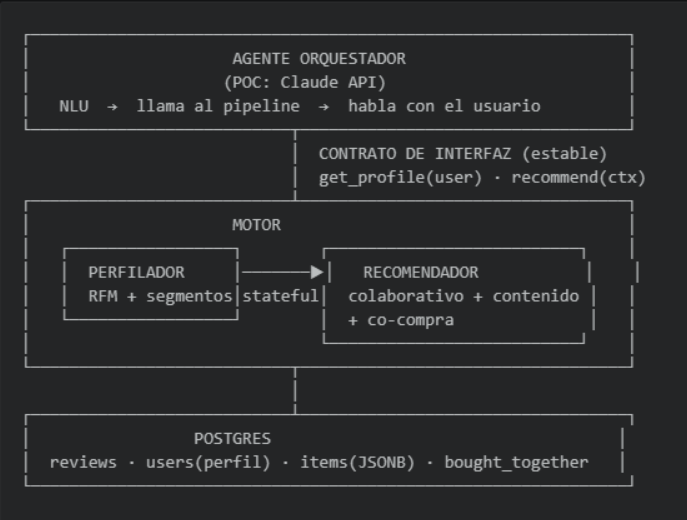
\includegraphics[width=.65\textwidth]{./Figuras/diagrama_basico.png}
\caption{Diagrama del sistema.}
\label{fig:diagrama_basico}
\end{figure}

El alcance de este trabajo se acota al diseño e implementación del sistema de perfilado-recomendación y de su API, sin abarcar el desarrollo del flujo conversacional completo; no obstante, se construirá una prueba de concepto que demuestre cómo un agente conversacional podría consumir dicha API en tiempo real. Entre los desafíos identificados a priori se destacan: el sesgo introducido por utilizar reseñas como proxy de compra (solo se observa al usuario cuando dejó una reseña), el problema de cold-start para usuarios e ítems nuevos, y la cobertura incompleta de metadata en parte del dataset, que se resolverá filtrando o marcando los ítems afectados según la estrategia de splitting estándar del dataset.

Se trata de un desarrollo desde cero que se llevará hasta el nivel de prueba de concepto; la innovación radica principalmente en el enfoque de transfer learning aplicado a la combinación perfilado-recomendación y en el diseño de una interfaz agnóstica al bot conversacional, lo que habilita su reutilización en distintos verticales de comercio.

\section{2. Identificación y análisis de los interesados}
\label{sec:interesados}

\begin{table}[ht]
\begin{tabularx}{\linewidth}{@{}|l|X|X|X|@{}}
\hline
\rowcolor[HTML]{C0C0C0}
Rol           & Nombre y Apellido & Organización 	& Puesto 	\\ \hline
Cliente       & \clientename      & \empclientename	& Referente de producto \\ \hline
Responsable   & \authorname       & FIUBA        	& Alumno 	\\ \hline
Orientador    & \supname	      & \pertesupname 	& Director del Trabajo Final \\ \hline
Usuario final & -                 & -            	& Consumidor de retail que compra vía canal conversacional \\ \hline
\end{tabularx}
\end{table}

A continuación se detallan las principales características de cada interesado:

\begin{itemize}
	\item Cliente: Equipo de IA Conversacional. Ofrece soluciones de compra conversacional a sus propios clientes. En este caso, de retail. Este interesado valora que el motor de perfilado-recomendación sea agnóstico al bot conversacional y a la vertical de comercio, de forma de poder reutilizarlo en distintas implementaciones para sus clientes.
	\item Responsable: el propio alumno, cursante de la Carrera de Especialización en Inteligencia Artificial de FIUBA, a cargo de la totalidad del diseño, desarrollo y documentación del proyecto.
	\item Orientador: a definir. Todavía no se cuenta con un director de Trabajo Final asignado.
	\item Usuario final: es un consumidor genérico de una tienda de retail que interactúa con el agente conversacional para buscar y comprar productos. No se ha caracterizado un segmento específico de usuario, ya que el sistema está pensado para ser agnóstico al vertical de comercio.
\end{itemize}


\section{3. Propósito del proyecto}
\label{sec:proposito}

Diseñar e implementar un sistema de perfilado y recomendación para retail, basado en un enfoque de transfer learning, que pueda integrarse como herramienta de un agente conversacional de compras. Se busca que el sistema perfile a los usuarios a partir de features RFM y de comportamiento, y que genere recomendaciones híbridas de productos con una calidad aceptable incluso contando con pocos datos propios del cliente que lo adopte, aprovechando el conocimiento transferido desde un modelo pre entrenado sobre un dataset público y extenso. Se trata de una prueba de concepto con la cual se pretende demostrar que es posible desacoplar la inteligencia de recomendación del canal conversacional específico. Este enfoque habilita su reutilización entre distintos bots y verticales de comercio. De esta manera, se espera avanzar en el desarrollo profesional del alumno dentro del área de inteligencia artificial conversacional.

\section{4. Alcance del proyecto}
\label{sec:alcance}

El proyecto incluye:
\begin{itemize}
	\item Diseño e implementación del módulo perfilador, basado en features RFM y atributos de comportamiento.
	\item Diseño e implementación del módulo recomendador híbrido (colaborativo + contenido + co-compra).
	\item Entrenamiento de un modelo pre entrenado sobre el dataset Amazon Reviews'23.
	\item Búsqueda y selección de un dataset más acotado, todavía no identificado, sobre el cual ajustar un modelo ``dedicado'' vía transfer learning, para validar la hipótesis de mejores recomendaciones con menos datos.
	\item Exposición de los resultados vía una API con contrato estable (por ejemplo \texttt{get\_profile}, \texttt{recommend}).
	\item Diseño del esquema de persistencia en Postgres (reviews, perfiles de usuario, ítems, co-compra).
	\item Una prueba de concepto de un agente conversacional simple que se monte sobre la API sobre Claude para denotar el punta a punta.
\end{itemize}

El presente proyecto no incluye:
\begin{itemize}
	\item El desarrollo del flujo conversacional completo ni de la interfaz de usuario final. Es decir, no es un desarrollo que se proponga entregar una solución conversacional punta a punta cerrada.
	\item La integración con un bot conversacional real de producción. Tampoco espera ser conectada a un bot específico.
	\item El despliegue en infraestructura productiva ni la operación continua del sistema.
\end{itemize}


\section{5. Supuestos del proyecto}
\label{sec:supuestos}

Para el desarrollo del presente proyecto se supone que:

\begin{itemize}
	\item El dataset Amazon Reviews'23 es suficientemente representativo del comportamiento de compra como para entrenar un modelo pre entrenado útil, a pesar de estar compuesto por reseñas y no por transacciones directas.
	\item Que va a ser posible encontrar o construir un dataset más acotado, con menor volumen o riqueza de atributos, adecuado para validar el enfoque de transfer learning.
	\item Que la infraestructura de cómputo personal (o de bajo costo) disponible es suficiente para entrenar los modelos propuestos dentro de los plazos del proyecto.
	\item Que el uso del dataset Amazon Reviews'23 y de la API de Claude no presenta restricciones legales o de licenciamiento que impidan su uso en este trabajo.
	\item Que no van a existir cambios significativos en la disponibilidad o el formato del dataset público durante el desarrollo del proyecto.
\end{itemize}

\section{6. Product Backlog}
\label{sec:backlog}

El Product Backlog debe organizarse en cuatro \textbf{\textit{\'{e}picas}} fundamentales del proyecto. Cada \'{e}pica debe contener al menos dos historias de usuario que describan funcionalidades clave.

El Product Backlog debe permitir interpretar cómo será el proyecto y su funcionalidad. Se deben indicar claramente las prioridades entre las historias de usuario y si hay alguna opcional.

Las historias de usuario deben ser breves, claras y medibles, expresando el rol, la necesidad y el propósito de cada funcionalidad. También deben tener una prioridad definida para facilitar la planificación de los sprints.

Cada historia de usuario debe incluir una ponderación en \textit{Story Points}, un número entero que representa el tama\~no relativo de la historia. El criterio para calcular los Story Points debe indicarse explícitamente.

Las historias deben seguir el formato: ``\textit{Como [rol], quiero [tal cosa] para [tal otra cosa]}''.

Las \'{e}picas deben estructurarse de la siguiente forma:

\begin{itemize}
  \item \textbf{\'{E}pica 1}
    \begin{itemize}
      \item HU1
      \item HU2
    \end{itemize}
  \item \textbf{\'{E}pica 2}
    \begin{itemize}
      \item HU3
      \item HU4
    \end{itemize}
  \item \textbf{\'{E}pica 3}
    \begin{itemize}
      \item HU5
      \item HU6
    \end{itemize}
  \item \textbf{\'{E}pica 4}
    \begin{itemize}
      \item HU7
      \item HU8
    \end{itemize}
\end{itemize}

\textbf{Reglas para definir historias de usuario:}
\begin{itemize}
  \item Ser concisas y claras.
  \item Expresarlas en términos cuantificables y medibles.
  \item No dejar margen para interpretaciones ambiguas.
  \item Indicar claramente su prioridad y si son opcionales.
  \item Considerar regulaciones y normas vigentes.
\end{itemize}

\section{7. Criterios de aceptación de historias de usuario}
\label{sec:criteriosAceptacion}

Los criterios de aceptación deben establecerse para cada historia de usuario, asegurando que se cumplan las condiciones necesarias para que la funcionalidad sea validada correctamente.

Cada historia debe tener criterios medibles, específicos y verificables. Deben permitir validar que se cumple con las necesidades del usuario.

Se estructuran de forma análoga a las \'{e}picas del backlog:

\begin{itemize}
  \item \textbf{\'{E}pica 1}
    \begin{itemize}
      \item Criterios de aceptación HU1
      \item Criterios de aceptación HU2
    \end{itemize}
  \item \textbf{\'{E}pica 2}
    \begin{itemize}
      \item Criterios de aceptación HU3
      \item Criterios de aceptación HU4
    \end{itemize}
  \item \textbf{\'{E}pica 3}
    \begin{itemize}
      \item Criterios de aceptación HU5
      \item Criterios de aceptación HU6
    \end{itemize}
  \item \textbf{\'{E}pica 4}
    \begin{itemize}
      \item Criterios de aceptación HU7
      \item Criterios de aceptación HU8
    \end{itemize}
\end{itemize}

\textbf{Reglas para definir criterios de aceptación:}
\begin{itemize}
  \item Medibles y verificables.
  \item Especificar cuándo una historia se considera completada.
  \item Incluir condiciones específicas.
  \item No ambiguos.
  \item Probables de testear funcional o técnicamente.
  \item Mínimo 3 criterios por HU.
\end{itemize}

\section{8. Fases de CRISP-DM}

\begin{enumerate}
  \item \textbf{Comprensión del negocio:} objetivo, valor agregado de IA, métricas de éxito.
  \item \textbf{Comprensión de los datos:} tipo, origen, cantidad, calidad.
  \item \textbf{Preparación de los datos:} características clave, transformaciones necesarias.
  \item \textbf{Modelado:} tipo de problema, algoritmos posibles.
  \item \textbf{Evaluación del modelo:} métricas de rendimiento.
  \item \textbf{Despliegue del modelo (opcional):} tipo de despliegue y herramientas.
\end{enumerate}

\section{9. Desglose del trabajo en tareas}
\label{sec:wbs}

A partir de cada Historia de Usuario (HU) definida en la sección 6, descomponer el trabajo en tareas técnicas concretas, medibles y acotadas en el tiempo.

\begin{itemize}
\item Seleccionar entre 2 y 3 tareas por cada historia de usuario.
\item Cada tarea debe estar claramente formulada, ser técnica, accionable y con una estimación horaria entre 2 y 8 horas.
\item Evitar tareas genéricas (como ''desarrollar funcionalidad´´) o demasiado amplias.
\item Si una tarea supera las 8 horas, debe dividirse en subtareas.
\item Indicar la prioridad relativa de cada tarea (Alta, Media o Baja).
\end{itemize}

\begin{table}[htpb]
\centering
\begin{tabularx}{\linewidth}{@{}|X|X|c|c|@{}}
\hline
\rowcolor[HTML]{C0C0C0}
Historia de usuario & Tarea técnica & Estimación & Prioridad \\ \hline
HU1 & Tarea 1 HU1 & 6 h & Alta \\ \hline
HU1 & Tarea 2 HU1 & 8 h & Alta \\ \hline
HU2 & Tarea 1 HU2 & 5 h & Media \\ \hline
HU2 & Tarea 2 HU2 & 6 h & Alta \\ \hline
... & ... & ... & ... \\ \hline
\end{tabularx}
\end{table}

\textbf{Criterios para estimar tiempos:}
\begin{itemize}
  \item Considerar la complejidad técnica, el nivel de incertidumbre y la experiencia previa.
  \item Evitar subestimar el esfuerzo: estimar el tiempo realista que llevaría implementar, testear y documentar cada tarea.
  \item Basar la estimación en la experiencia propia o en referencias de tareas similares.
\end{itemize}

\textbf{Sobre la prioridad:}
\begin{itemize}
  \item Asignar una prioridad relativa (Alta, Media o Baja) según la relevancia funcional de la tarea y su impacto en los entregables.
  \item Priorizar tareas que estén vinculadas a criterios de aceptación de las HU o que sean necesarias para desbloquear otras.
  \item Incluir tareas opcionales solo si están bien justificadas.
\end{itemize}

\textbf{Recomendaciones generales:}
\begin{itemize}
  \item -Enfocarse en tareas que surgen directamente de las HU planteadas.
  \item No es necesario cubrir las 600 horas del proyecto en esta sección: el foco está en el desglose de funcionalidades clave.
  \item Este trabajo será la base para organizar algunos de los sprints y elaborar el cronograma del proyecto, por lo que debe ser claro y realista.
\end{itemize}

\section{10. Planificación de Sprints}

Organizar las tareas técnicas del proyecto en sprints de trabajo que permitan distribuir de forma equilibrada la carga horaria total, estimada en 600 horas.

\textbf{Consigna:}
\begin{itemize}
  \item Completar una tabla que relacione sprints con HU y tareas técnicas correspondientes.
  \item Incluir estimación en horas para cada tarea.
  \item Indicar responsable y porcentaje de avance estimado o completado.
  \item Contemplar también tareas de planificación, documentación, redacción de memoria y preparación de defensa.
\end{itemize}

\textbf{Conceptos clave:}
\begin{itemize}
  \item Una \'{e}pica es una unidad funcional amplia; una historia de usuario es una funcionalidad concreta; un sprint es una unidad de tiempo donde se ejecutan tareas.
  \item Las tareas son el nivel más desagregado: permiten estimar tiempos, asignar responsables y monitorear progreso.
\end{itemize}

\textbf{Duración sugerida:}
\begin{itemize}
  \item Para un proyecto de 600 h, se recomienda planificar entre 10 y 12 sprints de aproximadamente 2 semanas cada uno.
  \item Asignar entre 45 y 50 horas efectivas por sprint a tareas técnicas.
  \item Reservar 100 a 120 h para actividades no técnicas (planificación, escritura, reuniones, defensa).
\end{itemize}

\textbf{Importante:}
\begin{itemize}
  \item En proyectos individuales, el responsable suele ser el propio autor.
  \item Aun así, desagregar tareas facilita el seguimiento y mejora continua.
\end{itemize}

\textbf{Conversión opcional de Story Points a horas:}
\begin{itemize}
  \item 1 SP \(\approx\) 2 h como referencia flexible.
  \item Tener en cuenta aproximaciones tipo Fibonacci.
\end{itemize}

\begin{table}[htpb]
\centering
\caption{Formato sugerido}
\begin{tabularx}{\linewidth}{@{}|l|l|X|c|l|c|@{}}
\hline
\rowcolor[HTML]{C0C0C0}
Sprint & HU o fase & Tarea & Horas / SP & Responsable & \% Completado \\ \hline
Sprint 0 & Planificación & Definir alcance y cronograma & 10 h & Alumno & 100\% \\ \hline
Sprint 0 & Planificación & Reunión con el tutor/cliente & 5 h & Alumno & 50\% \\ \hline
Sprint 0 & Planificación & Ajuste de los entregables & 6 h & Alumno & 25\% \\ \hline
Sprint 1 & HU1 & Tarea 1 HU1 & 6 h / 3 SP & Alumno & 0\% \\ \hline
Sprint 1 & HU1 & Tarea 2 HU1 & 10 h / 5 SP & Alumno & 0\% \\ \hline
Sprint 2 & HU2 & Tarea 1 HU2 & 7 h / 5 SP & Alumno & 0\% \\ \hline
... & ... & ... & ... & ... & ... \\ \hline
Sprint 5 & Escritura & Redacción memoria & 50 h / 34 SP & Alumno & 0\% \\ \hline
Sprint 6 & Defensa & Preparación de la exposición & 20 h / 13 SP & Alumno & 0\% \\ \hline
\end{tabularx}
\end{table}

\textbf{Recomendaciones:}
\begin{itemize}
  \item Verificar que la carga horaria por sprint sea equilibrada.
  \item Usar sprints de 1 a 3 semanas, acordes al cronograma general.
  \item Actualizar el \% completado durante el seguimiento del proyecto.
  \item Considerar un sprint final exclusivo para pruebas, revisión y ajustes antes de la defensa.
\end{itemize}


\section{11. Diagrama de Gantt (sprints)}
\label{sec:gantt}

Visualizar en un diagrama de Gantt la planificación temporal del proyecto, tomando como base los sprints definidos en la sección anterior. Debe contemplar todas las horas del proyecto.

Consigna:

\begin{itemize}

\item Elaborar un diagrama de Gantt que muestre la secuencia temporal de los sprints.

\item Cada fila debe representar un sprint (con su número o nombre), y el eje horizontal debe indicar el tiempo (en semanas o fechas concretas).

\item Las tareas técnicas derivadas de HU deben diferenciarse visualmente (por ejemplo, con un color distinto) de las tareas no técnicas (planificación, redacción, defensa).

\item Incluir todas las tareas estimadas en cada sprint.
\end{itemize}

Recomendaciones para el Gantt:

\begin{itemize}

	\item Podés usar herramientas gratuitas como TeamGantt, ClickUp, GanttProject, [Google Sheets], [Trello + Planyway], entre otras.
	\item Ordená los sprints de forma cronológica, comenzando con Sprint 0 (planificación) y finalizando con el sprint de defensa.
	\item Asegurate de reflejar la duración realista de cada sprint según tu disponibilidad y el cronograma general del posgrado.
	\item Incluí hitos importantes: reuniones, entregas parciales, defensa.
\end{itemize}


Incluir una imagen legible del diagrama de Gantt. Si es muy ancho, presentar primero la tabla y luego el gráfico de barras.



\section{12. Gobernanza de datos}
\label{sec:gobernanza}

En esta sección se debe analizar de manera integral el marco normativo y ético asociado al uso de los datos y al desarrollo de soluciones basadas en inteligencia artificial.

El análisis se divide en dos partes:

\begin{itemize}
  \item Cumplimiento normativo.
  \item Ética en el uso de inteligencia artificial.
\end{itemize}

\subsection{Cumplimiento normativo}
Este análisis es clave para garantizar el cumplimiento normativo y evitar conflictos legales durante el desarrollo y publicación del proyecto.

En esta subsección se debe identificar si los datos utilizados en el proyecto están sujetos a normativas de protección de datos y privacidad, y en qué condiciones pueden emplearse.

Aspectos a considerar:

\begin{itemize}
  \item Determinar si los datos están regulados por normativas como el GDPR, la Ley 25.326 de Protección de Datos Personales (Argentina), la HIPAA u otras, según la jurisdicción o la temática del proyecto.
  \item Aclarar si las fuentes de datos son propias, de acceso público o licenciadas. En este último caso, explicitar la licencia correspondiente y sus condiciones de uso. Realizar este mismo análisis para las herramientas y, en caso de corresponder, para los modelos preentrenados a emplear.
  \item Analizar la viabilidad legal del proyecto, considerando los mecanismos necesarios para garantizar el cumplimiento normativo y la trazabilidad de los datos.
\end{itemize}

\subsection{Ética en el uso de inteligencia artificial}

En esta subsección se debe reflexionar sobre los aspectos éticos vinculados al uso de datos y algoritmos de inteligencia artificial. Se espera una evaluación de la integridad del sistema y su impacto social.

Aspectos a considerar:

\begin{itemize}
	\item Identificar posibles sesgos en los datos o modelos (ideológicos, culturales, de género, geográficos, etc.) y analizar sus consecuencias (por ejemplo: discriminación, manipulación, pérdida de privacidad o desinformación).
	\item Analizar los posibles riesgos en términos de impacto social del uso indebido de la solución a desarrollar.
	\item En caso de corresponder, proponer medidas de mitigación y mecanismos de confianza (auditorías, documentación, trazabilidad, revisión humana, etc.).
	\item Finalmente, elaborar una reflexión general sobre la ética del proyecto, considerando tanto la equidad y transparencia del sistema como su impacto potencial en la sociedad.

\end{itemize}


\section{13. Gestión de riesgos}
\label{sec:riesgos}

\begin{consigna}{red}
a) Identificación de los riesgos (al menos cinco) y estimación de sus consecuencias:
 
Riesgo 1: detallar el riesgo (riesgo es algo que si ocurre altera los planes previstos de forma negativa)
\begin{itemize}
	\item Severidad (S): mientras más severo, más alto es el número (usar números del 1 al 10).\\
	Justificar el motivo por el cual se asigna determinado número de severidad (S).
	\item Probabilidad de ocurrencia (O): mientras más probable, más alto es el número (usar del 1 al 10).\\
	Justificar el motivo por el cual se asigna determinado número de (O). 
\end{itemize}   

Riesgo 2:
\begin{itemize}
	\item Severidad (S): X.\\
	Justificación...
	\item Ocurrencia (O): Y.\\
	Justificación...
\end{itemize}

Riesgo 3:
\begin{itemize}
	\item Severidad (S):  X.\\
	Justificación...
	\item Ocurrencia (O): Y.\\
	Justificación...
\end{itemize}


b) Tabla de gestión de riesgos:      (El RPN se calcula como RPN=SxO)

\begin{table}[htpb]
\centering
\begin{tabularx}{\linewidth}{@{}|X|c|c|c|c|c|c|@{}}
\hline
\rowcolor[HTML]{C0C0C0} 
Riesgo & S & O & RPN & S* & O* & RPN* \\ \hline
       &   &   &     &    &    &      \\ \hline
       &   &   &     &    &    &      \\ \hline
       &   &   &     &    &    &      \\ \hline
       &   &   &     &    &    &      \\ \hline
       &   &   &     &    &    &      \\ \hline
\end{tabularx}%
\end{table}

Criterio adoptado: 

Se tomarán medidas de mitigación en los riesgos cuyos números de RPN sean mayores a...

Nota: los valores marcados con (*) en la tabla corresponden luego de haber aplicado la mitigación.

c) Plan de mitigación de los riesgos que originalmente excedían el RPN máximo establecido:
 
Riesgo 1: plan de mitigación (si por el RPN fuera necesario elaborar un plan de mitigación).
  Nueva asignación de S y O, con su respectiva justificación:
  \begin{itemize}
	\item Severidad (S*): mientras más severo, más alto es el número (usar números del 1 al 10).
          Justificar el motivo por el cual se asigna determinado número de severidad (S).
	\item Probabilidad de ocurrencia (O*): mientras más probable, más alto es el número (usar del 1 al 10).
          Justificar el motivo por el cual se asigna determinado número de (O).
	\end{itemize}

Riesgo 2: plan de mitigación (si por el RPN fuera necesario elaborar un plan de mitigación).
 
Riesgo 3: plan de mitigación (si por el RPN fuera necesario elaborar un plan de mitigación).

\end{consigna}

\section{14. Sprint Review}
\label{sec:sprint_review}

La revisión de sprint (\emph{Sprint Review}) es una práctica fundamental en metodologías ágiles. Consiste en revisar y evaluar lo que se ha completado al finalizar un sprint. En esta instancia, se presentan los avances y se verifica si las funcionalidades cumplen con los criterios de aceptación establecidos. También se identifican entregables parciales y se consideran ajustes si es necesario.

Aunque el proyecto aún se encuentre en etapa de planificación, esta sección permite proyectar cómo se evaluarán las funcionalidades más importantes del backlog. Esta mirada anticipada favorece la planificación enfocada en valor y permite reflexionar sobre posibles obstáculos.

\textbf{Objetivo:} anticipar cómo se evaluará el avance del proyecto a medida que se desarrollen las funcionalidades, utilizando como base al menos cuatro historias de usuario del \emph{Product Backlog}.


Seleccionar al menos 4 HU del Product Backlog. Para cada una, completar la siguiente tabla de revisión proyectada:

\textbf{Formato sugerido:}
\begin{table}[htpb]
\renewcommand{\arraystretch}{1.5}
\begin{tabular}{|>{\raggedright\arraybackslash}m{2.4cm}|
                >{\raggedright\arraybackslash}m{2.3cm}|
                >{\raggedright\arraybackslash}m{3cm}|
                >{\raggedright\arraybackslash}m{3cm}|
                >{\raggedright\arraybackslash}m{3cm}|}
\hline
\rowcolor[HTML]{CCCCCC}
\textbf{HU seleccionada} & \textbf{Tareas asociadas} & \textbf{Entregable esperado} & \textbf{¿Cómo sabrás que está cumplida?} & \textbf{Observaciones o riesgos} \\
\hline
                         & Tarea 1 &                             &                                           &                                     \\ \cline{2-2}
\multirow{-2}{=}{HU1}    & Tarea 2 & \multirow{-2}{=}{Módulo funcional} & \multirow{-2}{=}{Cumple criterios de aceptación definidos} & \multirow{-2}{=}{Falta validar con el tutor} \\
\hline
                         & Tarea 1 &                             &                                           &                                     \\ \cline{2-2}
\multirow{-2}{=}{HU3}    & Tarea 2 & \multirow{-2}{=}{Reporte generado} & \multirow{-2}{=}{Exportación disponible y clara} & \multirow{-2}{=}{Requiere datos reales} \\
\hline
                         & Tarea 1 &                             &                                           &                                     \\ \cline{2-2}
\multirow{-2}{=}{HU5}    & Tarea 2 & \multirow{-2}{=}{Panel de gestión} & \multirow{-2}{=}{Roles diferenciados operativos} & \multirow{-2}{=}{Riesgo en integración} \\
\hline
                         & Tarea 1 &                             &                                           &                                     \\ \cline{2-2}
\multirow{-2}{=}{HU7}    & Tarea 2 & \multirow{-2}{=}{Informe trimestral} & \multirow{-2}{=}{PDF con gráficos y evolución} & \multirow{-2}{=}{Puede faltar tiempo para ajustes} \\
\hline
\end{tabular}
\end{table}

\section{15. Sprint Retrospective}    
\label{sec:sprint_retro}

La retrospectiva de sprint es una práctica orientada a la mejora continua. Al finalizar un sprint, el equipo (o el alumno, si trabaja de forma individual) reflexiona sobre lo que funcionó bien, lo que puede mejorarse y qué acciones concretas pueden implementarse para trabajar mejor en el futuro.

Durante la cursada se propuso el uso de la \textbf{Estrella de la Retrospectiva}, que organiza la reflexión en torno a cinco ejes:

\begin{itemize}
\item  ¿Qué hacer más?
\item  ¿Qué hacer menos?
\item  ¿Qué mantener?
\item  ¿Qué empezar a hacer?
\item  ¿Qué dejar de hacer?
\end{itemize}

Aun en una etapa temprana, esta herramienta permite que el alumno planifique su forma de trabajar, identifique anticipadamente posibles dificultades y diseñe estrategias de organización personal.

\textbf{Objetivo:} reflexionar sobre las condiciones iniciales del proyecto, identificando fortalezas, posibles dificultades y estrategias de mejora, incluso antes del inicio del desarrollo.


Completar la siguiente tabla tomando como referencia los cinco ejes de la Estrella de la Retrospectiva (\emph{Starfish} o estrella de mar). Esta instancia te ayudará a definir buenas prácticas desde el inicio y prepararte para enfrentar el trabajo de forma organizada y flexible. Se deberá completar la tabla al menos para 3 sprints técnicos y 1 no técnico.

\textbf{Formato sugerido:}

\begin{table}[htpb]
\renewcommand{\arraystretch}{1.4}
\begin{tabular}{|>{\raggedright\arraybackslash}p{1.8cm}|
                >{\raggedright\arraybackslash}p{2.3cm}|
                >{\raggedright\arraybackslash}p{2.3cm}|
                >{\raggedright\arraybackslash}p{2.3cm}|
                >{\raggedright\arraybackslash}p{2.3cm}|
                >{\raggedright\arraybackslash}p{2.3cm}|}
\hline
\rowcolor[HTML]{CCCCCC} 
\textbf{Sprint tipo y N°} & \textbf{¿Qué hacer más?} & \textbf{¿Qué hacer menos?} & \textbf{¿Qué mantener?} & \textbf{¿Qué empezar a hacer?} & \textbf{¿Qué dejar de hacer?} \\
\hline
Sprint técnico - 1 & Validaciones continuas con el alumno & Cambios sin versión registrada & Pruebas con datos simulados & Documentar cambios propuestos & Ajustes sin análisis de impacto \\
\hline
Sprint técnico - 2 & Verificar configuraciones en múltiples escenarios & Modificar parámetros sin guardar historial & Perfiles reutilizables & Usar logs para configuración & Repetir pruebas manuales innecesarias \\
\hline
Sprint técnico - 8 & Comparar correlaciones con casos previos & Cambiar parámetros sin justificar & Revisión cruzada de métricas & Anotar configuraciones usadas & Trabajar sin respaldo de datos \\
\hline
Sprint no técnico - 12 (por ej.: ``Defensa'') & Ensayos orales con feedback & Cambiar contenidos en la memoria & Material visual claro & Dividir la presentación por bloques & Agregar gráficos difíciles de explicar \\
\hline
\end{tabular}
\end{table}




\end{document}
